\chapter{EXPERIMENTAL PROCEDURE}
\label{ch:experimental-procedure}

% \begin{center}\textit{Alphas have more mass because they spend so much
% time at the gym getting swole. \---{} Laura Moran}\end{center}

To support the commissioning work of St.\ George through using reaction
measurements, and to explore the possibility of extending the use cases
of the separator beyond $(\alpha,\gamma)$ reactions, the well-studied
\alpa{} reaction was chosen to be an initial test case. The properties
of the reaction can be used to verify the desired properties of the
separator under a reaction study, effectively emulating the conditions
under which the initially proposed $(\alpha,\gamma)$ reactions will be
performed.

To this end, an experimental campaign to study the \alpa{} reaction with
the St.\ George recoil separator was undertaken at the NSL. Runs were
completed in December 2016 and February 2017, with runs focusing on
determining the correct magnetic fields within St.\ George completed in
Fall 2016 and February 2017. Two low energy resonances were measured
with beam currents in the $2-3$~$\mu$A range in February 2017. Studying
this reaction provides a test of the angular and energy acceptances of
St.\ George in preparation for studying $(\alpha,\gamma)$ reactions
across a wide range of targets and energies.

The first portion of these runs fall under general St.\ George
commissioning work as discussed in Chapter~\ref{ch:commissioning} and
will not be repeated here. The second portion of the runs involved
characterizing the target and the detector, finalizing the optimal
settings for the separator, and performing the experiment. The reaction
of interest produces $\alpha$ particles in the energy range of $2-3$~MeV
for the desired proton energy range.


\section{Altered Tune}

The magnet settings for St.\ George were determined to transport
$\alpha$ particles from within a 40~mrad angular acceptance cone and
with at least a 2\,\% energy acceptance. As the produced $\alpha$
particles have a larger angular emittance than what can be transported
by St.\ George, only those particles emitted within the desired 40~mrad
acceptance cone for St.\ George were tuned to reach the detector focal
plane $F_2$ after the Wien filter and impinge the installed Si strip
detector.

The restrictions on the beam spot for measuring $(\rm{p},\alpha)$
reactions at this focal plane require an approximately symmetric spot
size in both directions and one that is smaller than the physical face
of the detector, whereas the standard tune for studying
$(\alpha,\gamma)$ reactions required that beam spot to be asymmetric
with the beam spot being narrow in the dispersive $x$-plane and tall in
the $y$-plane. The initial COSY code for St.\ George (see
Section~\ref{sec:cosy}) was altered to model the shortened separator and
provide information on the beam characteristics at the new detector
focal plane. The magnetic field settings for the seven quadrupoles
$Q_{1-7}$ were adjusted to transport the recoil particles to the
detector plane with a final beam spot no larger than the face of the Si
detector of $58\times 58$~mm. Final pole tip fields are given in
Table~\ref{tab:poletip}.

For the $(\rm{p},\alpha)$ experiment, the transported $\alpha$ particles
have the properties listed in Table~\ref{tab:alpha_prop}. The incident
proton beam is rejected within the COSY ion optics solution after the
first dipole doublet $B_1B_2$, and the beam properties are not listed
here.

\begin{table}
    \begin{center}
        \caption{POLE TIP FIELDS FOR $(\alpha,\gamma)$ AND
            $(\rm{p},\alpha)$ STUDIES}
        \label{tab:poletip}
        \begin{tabular}{cS[table-format=2.9]S[table-format=3.6]}
            \toprule
            \midrule
             & \multicolumn{2}{c}{\textbf{Pole Tip Field [T]}} \\
            \textbf{Quadrupole} & {$(\alpha,\gamma)$} &
            {$(\rm{p},\alpha)$} \\
            \midrule
            1  & -0.16303276 & -0.157\\
            2  &  0.18882363 &  0.187\\
            3  &  0.09384148 &  0.09411\\
            4  & -0.12620402 & -0.04\\
            5  &  0.10032405 &  0.092 \\
            6  &  0.04693654 &  0.0585 \\
            7  &  0.0        & -0.015 \\
            8  & -0.09779179 & \\
            9  &  0.17439627 & \\
            10 &  0.21092228 & \\
            11 & -0.13962355 & \\
            \bottomrule
        \end{tabular}
    \end{center}
\end{table}

\begin{table}
    \begin{center}
        \caption{ALPHA PARTICLE PROPERTIES}
        \label{tab:alpha_prop}
        \begin{tabular}{cc}
            \toprule
            \midrule
            \textbf{Property [Unit]} & \textbf{Value} \\
            \midrule
            Average Energy [MeV]  & 2.504 \\
            $\Delta$Energy [\%]   & 3 \\
            Angular spread [mrad] & 40 \\
            Target diameter [mm]  & 3 \\
            $Q$ [$e$]             & 2 \\
            $B\rho$ [Tm]          & 0.228 \\
            $E\rho$ [MV]          & 4.0 \\
            \bottomrule
        \end{tabular}
    \end{center}
\end{table}

\subsection{Separator Properties}

The energy resolving power is the minimum energy difference required to
resolve a peak from the central image peak assuming that the change in
energy is the only difference between the two peaks. By definition this
quantity is only a first-order value, so only those parameters with a
linear relationship with the position need be considered. The energy
resolving power of the separator in relation to the terms present in the
COSY transport map is defined as
\begin{equation}
    \delta_k(\textrm{RP}) \equiv
        \frac{2\left[(x|x)x_0 + (x|a)a_0\right]}{(x|\delta_k)},
\end{equation}
where $x_0$ and $a_0$ are the initial half-widths for position (in
meters) and angle (in radians), respectively, and the remaining terms
are the values from the transport map. The resolving power is only taken
in the horizontal plane due to the vertical symmetry of the separator.
The terms taken from the transport map are
\begin{align*}
    (x|x) &= 2.261610 \\
    (x|a) &= {-0.1368242} \\
    (x|\delta_k) &= {-0.2774295},
\end{align*}
where signs are conserved for completeness. The maximal deviation caused
by each terms is taken to be a positive value. The half-widths $x_0$ and
$a_0$ are physically limited by the target chamber and taken to be $x_0
= 1.5$~mm and $a_0 = 42$~mrad, giving a resolving power of
$\delta_k(\textrm{RP}) = 0.286$. Since the produced $\alpha$ particles
have an inherent spread in energy due to the incoming beam and the
particles themselves interacting with the target, the energy resolution
should be viewed as the window within which the energies are
indistinguishable. As this window covers the expected energy spread of
the produced $\alpha$ particles, there are no energy corrections
required across the detector strips.

Beam currents at the target location were recorded before and after each
run. For runs lasting longer than 15 minutes, the current was recorded
every 15 minutes. The beam current was seen to fluctuate around the
recorded value by up to 100~nA. For runs with multiple current readings,
the average was taken as the nominal current. Time on target was
recorded by the acquisition system.

\subsection{Beam Reduction}

% Glenlivet 12 Year

Incident proton beam reduction on the order of $10^{10} - 10^{14}$ is
necessary in order to avoid damaging the Si detector and to allow for
the desired alpha peak to be detected. This reduction factor becomes
more important for those off-resonance runs where the count rate of the
produced $\alpha$ particles is much lower.

Due to the location of the Si detector at the post-Wien filter focal
plane $F_2$, incident beam reduction can only be achieved through the
tuning of the separator. In experiments that use the full length of
St.\ George, beam rejection can be obtained through the use of the mass
slits at $F_2$ to stop the beam after the Wien filter. The location of
these slits is the same location as the Si detector, eliminating their
use in this experiment. Due to the larger $\Delta m$ and $\Delta E$
between the incident proton beam and the produced $\alpha$ particles,
the incident beam is adequately reduced at this point by the dipole
magnets and Wien filter.

The Si detector provides the last stage of rejection for the incident
beam. Due to the energy difference between the protons and $\alpha$
particles, the particle peaks will be well separated in the energy
spectra. Low energy tails of the $\alpha$ peak observed during the
energy calibration runs do not have a large effect on the ability to
reject the remainder of the incident beam.


\section{Run Procedure}

For each experimental run, we aim to measure the experimental yield at
the detector in order to compare it to the theoretical yield for a given
angular and energy acceptance. The experimental yield is dependent on
the beam current, the run time, and the target properties. For each run,
the incident beam must be prepared, and the tuning of St.\ George must
match the expected energy of the produced $\alpha$ particles. Auxiliary
runs are performed to ensure that the beam rejection is within an
acceptable range, that the produced particle current is not too high,
and that the beam spot on the detector is centered. Once all of the
preparations are complete, a run at the desired energy can be performed.
All data was collected by the DAQ and stored as binary files for later
processing.

\begin{figure}
    \begin{center}
        \centerline{
            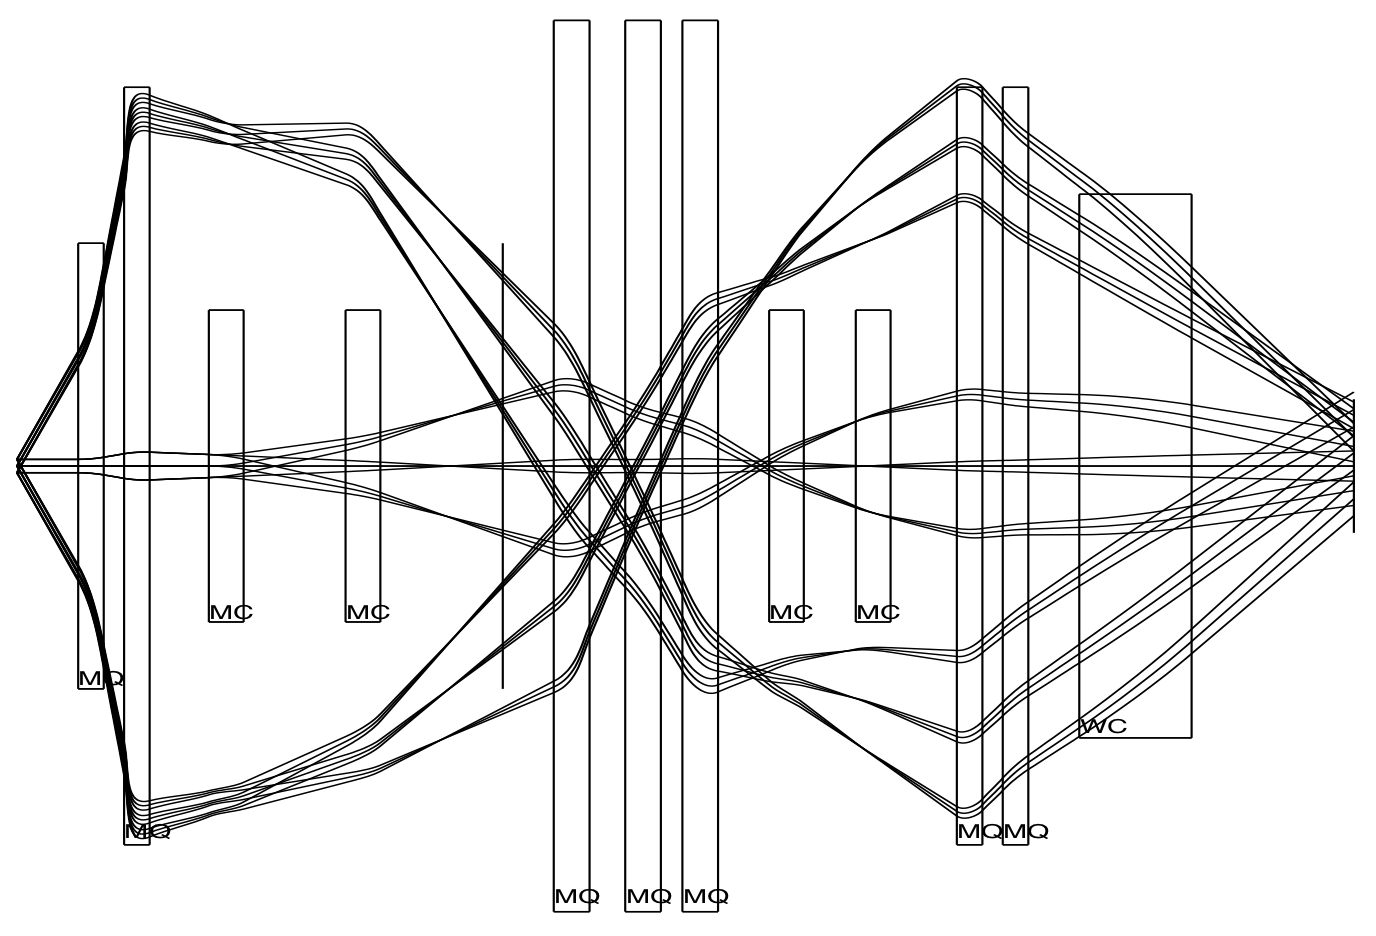
\includegraphics[width=0.8\textwidth]{figures/optimal_tune_x.png}}
        \centerline{
            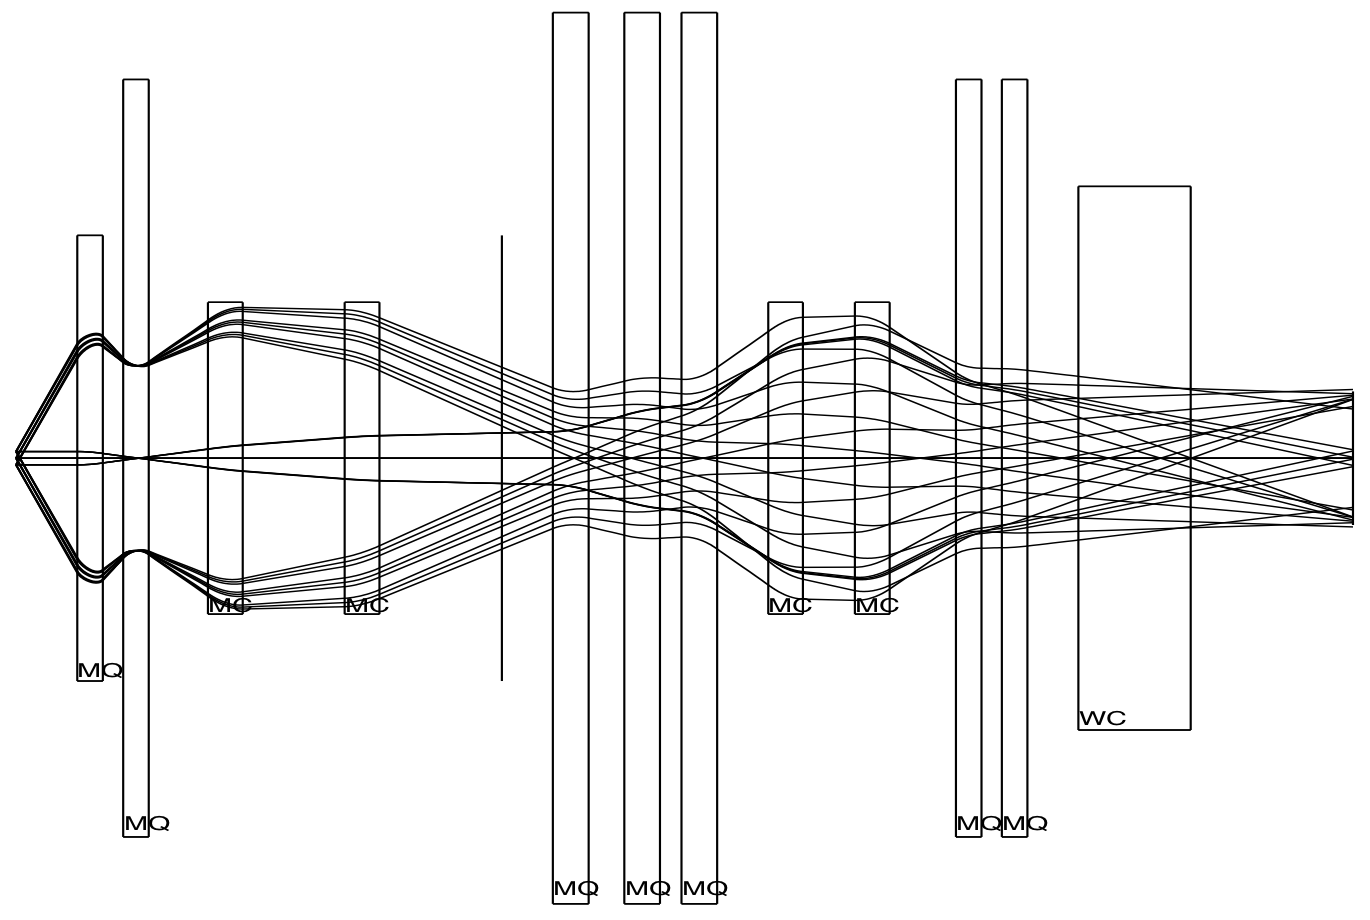
\includegraphics[width=0.8\textwidth]{figures/optimal_tune_y.png}}
        \caption[Horizontal and vertical rays through St.\
            George for $\alpha$ particles]{Horizontal (upper plot) and
            vertical (lower plot) rays through St.\ George for the
            altered tune transporting $\alpha$ particles to the
            post-Wien filter focal plane $F_2$. Only the $\alpha$
            particles are shown for simplicity. The pole tip fields are
            given in Table~\ref{tab:poletip}.}
        \label{fig:raytrace-altered}
    \end{center}
\end{figure}

The process below describes the steps taken for each individual energy
point. For each energy point, multiple runs are performed, with the
final run taking place with the final separator settings. The magnetic
settings for St.\ George are based on an altered tune to transport the
$\alpha$ particles to the Wien filter focal plane $F_2$ such that the
beam spot of the produced $\alpha$ particles is contained within the
physical extent of the Si detector. The desired rays through St.\ George
are shown in Fig.~\ref{fig:raytrace-altered}

The initial St.\ George magnetic settings were first found in a similar
manner to the energy and angular acceptance commissioning, with the
primary difference being the initial COSY settings for the magnets.

\newpage
\subsection{Beam Preparation}

The incident proton beam must be tuned for the desired energy. The beam
energy is set by adjusting the 5U and the analyzing magnet, with the
remainder of the transport beam line adjusted for the new energy. In
situations where the previous energy is close (within a few keV) to the
desired energy, this energy change is relatively straightforward as it
requires smaller changes to the beam line settings.

The incident beam must also be aligned with the magnetic optical axis of
St.\ George in the same manner as described in Sec.~\ref{sec:tuning}.
The magnets at the entrance of St.\ George, namely $Q_1Q_2B_1$ must be
brought down to zero in order to align the incident beam. The collimator
position is also determined in the same manner as the commissioning work
in order to determine the position of the Al target.

Once the beam is aligned, the target is put in place and $Q_1Q_2B_1$ are
recycled and brought to their scaled values for the $\alpha$ particle
energy in question. The recycling procedure ensures that the magnetic
field produced by the magnet is not affected by self-magnetization.

\subsection{Measuring Beam Suppression}

Once the incident beam is prepared, the next step is to see how much of
the beam reaches the detector plane without the target in place. This
step is a direct measurement of the suppression of the separator and is
essential to ensuring that the count rate at the detector due to the
beam is minimal. If the beam current at the detector due to the beam is
too high, it is possible that the detector could be damaged or the
signal of the produced $\alpha$ particles could be lost due to dead time
considerations.

The detector at the focal plane is located behind a thin Al shield when
fully retracted. This shield protects the exposed detector in situations
where the direct beam is incident through St.\ George. To determine if
the residual beam current at the detector plane is too high, the
detector is slowly moved up while the data acquisition system is
running. If the count rate is negligible, the detector is slowly moved
up in steps until it reaches its final position centered on the magnetic
optical axis.

Using the beam current at the target location, the suppression can be
calculated from the yield of the incident proton beam at the detector
plane. This suppression does not include the target effects, so it can be
considered as an initial estimate of the rejection of the separator. The
rejection is calculated by
\[
    S = \frac{N_{\rm beam at target}}{N_{\rm beam at detector}}.
\]
Initial measurements of the suppression of St.\ George for the altered
tune are approximately $10^{13}$. Once the suppression is determined to
be adequate for the experiment, the detector is again retracted to
behind the shield. The beam at this point is stopped before the target
location to allow for the moving of the detector and target.

\subsection{Target Effects}

The initial beam suppression does not include the effects of the target
on the incident beam. Once the initial suppression has been shown to be
acceptable for the detector, the target is placed into the beam line.
Its position is based on the found collimator position from the initial
beam tuning and alignment.

Once the target is in place, the detector will see $\alpha$ particles
produced in the reaction and any residual beam protons that are
transported to the focal plane. When the beam energy is on resonance,
there is a possibility that the produced $\alpha$ particle count rate is
high enough that there could be damage to the detector when combined
with the potential residual beam. With the detector still behind the
shield, the beam is sent into the target chamber.

As before, the detector is slowly moved up while monitoring the total
count rate at the detector. This count rate will primarily be due to the
produced $\alpha$ particles. Once the detector is fully extended, the
initial production runs to fine tune the settings of St.\ George can be
completed.

\subsection{Final Optimization}

When scaling the elements of St.\ George to the expected $\alpha$
particle energy, both the magnetic elements and the electrostatic plates
of the Wien filter need to be adjusted. The Wien filter voltage is set
according to
\[
    V_{\rm WF} = \frac{d E_{\alpha}}{2 \rho_{\rm WF}},
\]
where $d$ is the distance between the Wien filter plates in meters and
$\rho_{\rm WF}$ is the desired bending radius of the Wien filter. When
the $\alpha$ energy is given in keV, the final voltage will be in kV and
is the set point for each of the two electrodes.

The final Wien filter voltage may differ from this value. The central
energy of the $\alpha$ particles may be slightly different than that
used, the physical electrodes may have slight imperfections which change
the resulting electric field, or the voltage supplied to the
electrostatic plates may be slightly different than the set point. For
these reasons, the final tuning of the Wien filter is to center the
$\alpha$ particle count distribution horizontally on the Si detector.
Adjusting the Wien filter voltage to higher (lower) values for a set
magnetic field strength will move the $\alpha$ distribution right (left)
in the horizontal plane. An example showing the horizontal
distribution of the $\alpha$ particles is given in
Fig.~\ref{fig:alpha-distribution-strips}.

\begin{figure}
    \begin{center}
        \centerline{
            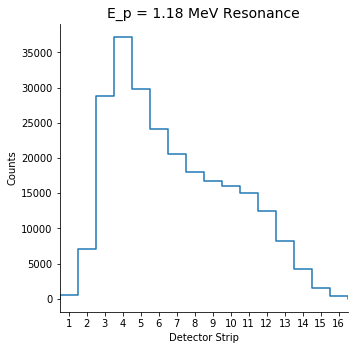
\includegraphics[width=0.6\textwidth]{figures/low_resonance_detector_strips.png}}
        \centerline{
            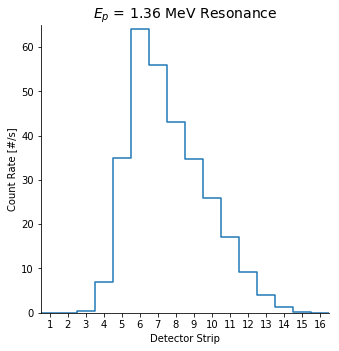
\includegraphics[width=0.6\textwidth]{figures/high_resonance_detector_strips.png}
        }
        \caption[Horizontal $\alpha$ particle distribution]{Horizontal
            $\alpha$ particle distribution at the detector plane after
            the Wien filter settings are optimized. The optimization
            centers the count distribution on the detector by adjusting
            the voltage to swing the beam distribution left or right.
            The runs near each of the resonance peaks are shown. Strip 1
            is on the ``beam right'' side of the detector.}
        \label{fig:alpha-distribution-strips}
    \end{center}
\end{figure}

\newpage
The $\alpha$ particle distribution potentially extends past the physical
limits of the Si detector in the horizontal and vertical direction.
Centering the distribution horizontally may still miss a small
proportion of counts. For runs that are near the resonance energy, the
counts missed horizontally is a minuscule fraction of the total counts
detected and can be effectively ignored. For runs at energies further
from the resonance energy, the fraction of counts that are missed by the
detector may become a larger fraction of the total counts, requiring
further studies to fully quantify the lost counts. The maximum expected
lost counts is around 1\,\% for our runs furthest from the resonance
energy. Since the acceptance of St.\ George is based on counts reaching
the detector, these lost counts are based on the tune of the separator
and provide an additional metric to measure the capabilities of the
separator.

An additional source of lost counts are those from the $\alpha$
distribution that reach the detector plane above and below the detector.
Due to the limitations of the detector system, only those counts below
the final detector position can be directly measured. As St.\ George is
vertically symmetric, we assume that the count rate above the detector
position is equal to that below the detector system. To measure these
counts below the detector position, the detector is moved down to the
position where the top of the Si detector is at the same vertical
position as the bottom of the detector when it is in its final position.
A figure displaying these positions is shown in
Fig.~\ref{fig:det-position}

Once these final checks are performed, the detector is returned to its
final position in the center of the beam line. At this point, the actual
measurement of the reaction yield can be measured.

\begin{figure}
    \begin{center}
        \centerline{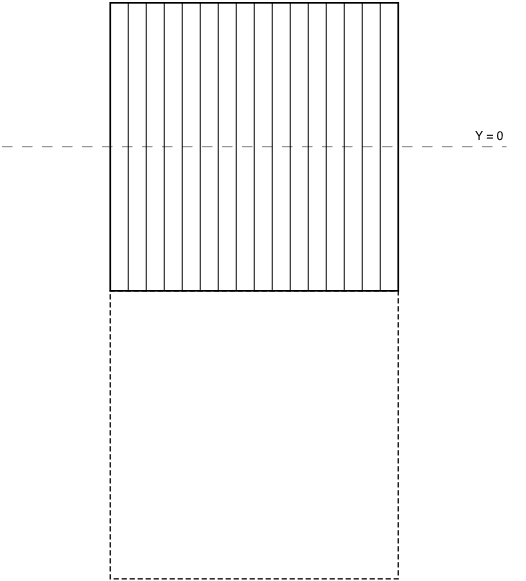
\includegraphics[width=0.8\textwidth]{figures/detector_position.png}}
        \caption[Detector positions]{Detector positions used to measure
            the produced $\alpha$ particles that miss the detector. The
            horizontal missed particles are determined through adjusting
            the Wien filter electrostatic field, since the horizontal
            position of the detector cannot be changed. The individual
            Si strips are vertical, so the actual vertical extent of the
            beam cannot be directly determined. The solid detector is
            the running position, which is centered vertically on the
            beam line. The dashed position is the low detector position
            used to estimate the vertical extent of the beam.}
        \label{fig:det-position}
    \end{center}
\end{figure}

\newpage
\subsection{Experimental Run}

At each energy, the yield of the produced $\alpha$ particles at the
detector is measured until a given threshold is met. For runs at or near
the resonance energy, data was collected for 15 minutes. The minimum run
time used reduces the possibility that minor fluctuations in the beam
current during the run have an outsized effect on the final yield. For
runs away from the resonance energy, the run was ended once
approximately 20k counts were detected within the expected energy range
of the produced $\alpha$ particles summed across all 16 Si strips. This
minimum count threshold ensures that the statistical uncertainty due to
the counts is less than 1\,\%.

For the final run, the incident beam current and the detector yield are
monitored throughout the run. A beam current measurement is taken before
and after the run to provide an estimate on the beam current during the
entire run. If the run continues for longer than 15 minutes, the current
is also measured every 15 minutes. Due to the design of the target
chamber without an offset Si detector, these periodic beam current
measurements are the only way to infer the changing beam current during
the run that is independent of the counts at the detector. As the beam
is not reacting with the target during these measurements, the time
taken is reduced from the total run time.

Once the run is completed, the beam is stopped and the system\---{}the
5U accelerator, the transport beam line, and St.\ George\---{}are
adjusted for the energy for the next run and the process is repeated.
